
\documentclass{beamer}

%\useoutertheme[glossy]{wuerzburg}
\useinnertheme[shadow,outline]{chamfered}
%\usecolortheme{shark}
\usecolortheme{beaver}
\beamertemplatenavigationsymbolsempty

\usefonttheme{professionalfonts}
\let\digamma\relax
\usepackage[scale=0.85,stdmathitalics=true,romanfamily=casual]{lucimatx}
\usefonttheme[stillsansseriftext]{serif}

\usepackage{bm}


\usepackage{fancyvrb}



\usepackage{textfit} % commands \scaletoheight{height}{text} and \scaletowidth{width}{text}

\usepackage{tikz}

\usepackage{tcolorbox}

\newtheorem{Alert}{Alert}
\newtheorem{Highlight}{Highlight}

\newcommand{\Species}[1]{{\rmfamily \itshape #1}}
\newcommand{\Real}{\ensuremath{\mathbb{R}}}
\newcommand{\RealN}{\ensuremath{\mathbb{R}^n}}
\newcommand{\RealP}{\ensuremath{\mathbb{R}^p}}
\newcommand{\Mtx}[1]{\ensuremath{\bm{#1}}}
\newcommand{\Inv}[1]{\ensuremath{#1^{-1}}}
\newcommand{\InvMtx}[1]{\ensuremath{\bm{#1}^{-1}}}
\newcommand{\Red}[1]{\textcolor{red}{#1}}
\newcommand{\PsInv}[1]{\ensuremath{\bm{#1}^{+}}}

\usepackage{booktabs}



% --- Macro \xvec
% From a tex.stackexchange.com answer by Todd Lehman
% http://tex.stackexchange.com/questions/44017/dot-notation-for-derivative-of-a-vector
\makeatletter
\newlength\xvec@height%
\newlength\xvec@depth%
\newlength\xvec@width%
\newcommand{\xvec}[2][]{%
  \ifmmode%
    \settoheight{\xvec@height}{$#2$}%
    \settodepth{\xvec@depth}{$#2$}%
    \settowidth{\xvec@width}{$#2$}%
  \else%
    \settoheight{\xvec@height}{#2}%
    \settodepth{\xvec@depth}{#2}%
    \settowidth{\xvec@width}{#2}%
  \fi%
  \def\xvec@arg{#1}%
  \def\xvec@dd{:}%
  \def\xvec@d{.}%
  \raisebox{.2ex}{\raisebox{\xvec@height}{\rlap{%
    \kern.05em%  (Because left edge of drawing is at .05em)
    \begin{tikzpicture}[scale=1]
    \pgfsetroundcap
    \draw (.05em,0)--(\xvec@width-.05em,0);
    \draw (\xvec@width-.05em,0)--(\xvec@width-.15em, .075em);
    \draw (\xvec@width-.05em,0)--(\xvec@width-.15em,-.075em);
    \ifx\xvec@arg\xvec@d%
      \fill(\xvec@width*.45,.5ex) circle (.5pt);%
    \else\ifx\xvec@arg\xvec@dd%
      \fill(\xvec@width*.30,.5ex) circle (.5pt);%
      \fill(\xvec@width*.65,.5ex) circle (.5pt);%
    \fi\fi%
    \end{tikzpicture}%
  }}}%
  #2%
}
\makeatother

% --- Override \vec with an invocation of \xvec.
\let\stdvec\vec
\renewcommand{\vec}[1]{\xvec[]{\bm{#1}}}
% --- Define \dvec and \ddvec for dotted and double-dotted vectors.
\newcommand{\dvec}[1]{\xvec[.]{#1}}
\newcommand{\ddvec}[1]{\xvec[:]{#1}}


\usepackage{pifont}
\newcommand{\weblink}{\ding{43}}  % hand with pointing finger

\definecolor{links}{HTML}{2A1B81}
\hypersetup{colorlinks,linkcolor=,urlcolor=magenta}

\usepackage{amsmath}
\usepackage{pdfpages}

\usepackage{tikz}
\newcommand*\circled[1]{\tikz[baseline=(char.base)]{
            \node[shape=circle,draw,inner sep=2pt] (char) {#1};}}

\parskip=0.5em

%===========================================================
\title{Introduction to Clustering}

\author{Paul M. Magwene}
\date{}


\begin{document}

\begin{frame}
\titlepage
\end{frame}


%===========================================================
\begin{frame}
  \frametitle{What is Clustering?}

``Clustering'' is a broad term for algorithms in statistics and machine learning
that try to discover ``natural groups'' in data.

What's a ``natural group''?


\begin{itemize}
  \item Common sense definition: Groups of objects (or variables) where similarity between objects is higher within groups than between groups
\end{itemize}

\end{frame}
%===========================================================


%===========================================================
\begin{frame}
  \frametitle{Natural Groups: Geometric Perspective}

What's a ``natural group''?

\begin{itemize}
  \item Geometric definition: Patches of high density points surrounded by patches of lower density in the $p$-dimensional space defined by the variates.
\end{itemize}

\begin{center}
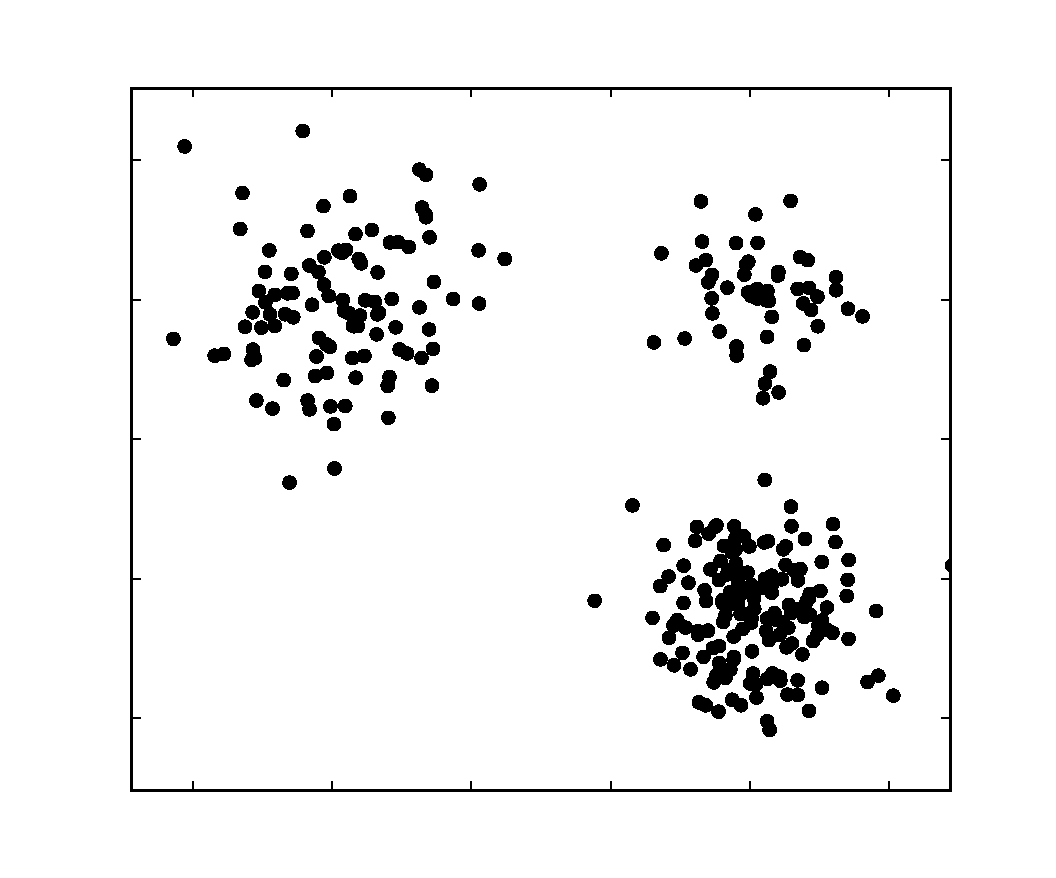
\includegraphics[height=1.5in]{cluster-fig.pdf}
\end{center}

\end{frame}
%===========================================================

%===========================================================
\begin{frame}
  \frametitle{Similarity/Dissimilarity}

\begin{block}{Intuition}
Similarity is a measure of ``likeness'' between two entities of interest. Dissimilarity is the complement of similarity.
\end{block}


\begin{itemize}

\item Dissimilarities may be converted to similarities (and vise versa) by taking any monotonically decreasing function. For example:
\[
s = 1 - d_{ij}  \ \mbox{(for $0 \leq d_{ij} \leq 1$)}
\]

\item Dissimilarities are usually in range $0 \leq d_{ij} \leq C$ where $C$ is the maximum dissimilarity

\item Distances are one measure of dissimilarity but distances are unbounded to the right
\[
d_{ij} \in [0,\infty]
\]
\end{itemize}
\end{frame}
%===========================================================

%===========================================================
\begin{frame}
  \frametitle{Dissimilarity Measures for Quantitative Data}

This simplest measure of dissimilarity is Euclidean distance.


\[
d_{ij} = \left\{ \sum_{k=1}^p (x_{ik} - x_{jk})^2 
         \right\} ^{1/2}
\]


\end{frame}
%===========================================================

%===========================================================
\begin{frame}
  \frametitle{Dissimilarity Measures for Quantitative Data, cont.}


\begin{itemize}

\item Manhattan (taxi cab, city block) distance
\[
d_{ij} = \sum_{k=1}^p | x_{ik} - x_{jk} |         
\]

\item Chebychev distance
\[
d_{ij} = max_k \left\{ | x_{ik} - x_{jk} | \right\}
\]

\item Minkowski Metric
\[
d_{ij} = \left\{ \sum_{k=1}^p |x_{ik} - x_{jk}|^\lambda
         \right\} ^{1/ \lambda}
\]

$\lambda = 1$ is Manhattan distance, $\lambda = 2$ is Euclidean distance, $\lambda = \infty$ is Chebychev distance.

\end{itemize}
\end{frame}
%===========================================================


%===========================================================
\begin{frame}
  \frametitle{Dissimilarity Measures for Variables}

Correlation provides a suitable measure of \emph{similarity}. 
Common \emph{dissimilarity} measures based on correlation include:


\begin{itemize}

\item $d_{kl} = 1 - r_{kl}$ if $r_{kl} = -1$ is taken to indicate maximum disagreement

\item $d_{kl} = 1 - r_{kl}^2$ if $r_{kl} = 1$ and $r_{kl} = -1$ are treated equivalently (predictive power)


\item Based on uncentered correlation:
\[
d_{kl} = 1 - \frac{\sum_{i=1}^n x_{ik}x_{il}} {\sum_{i=1}^n x_{ik}^2 \sum_{i=1}^n x_{il}^2}
\]

\end{itemize}
\end{frame}
%===========================================================


%===========================================================
\begin{frame}[plain,c]
\begin{center}
\Huge Hierarchical Clustering
\end{center}
\end{frame}
%===========================================================


%===========================================================
\begin{frame}[fragile]
  \frametitle{Clustering Method: Hierarchical Clustering}

For $n$ data points define a set of $n-1$ ``joins'' that represent
the groupings of objects at different levels of similarity. Represent
the series of joins as a ``tree'' graph.

\smallskip

\begin{center}
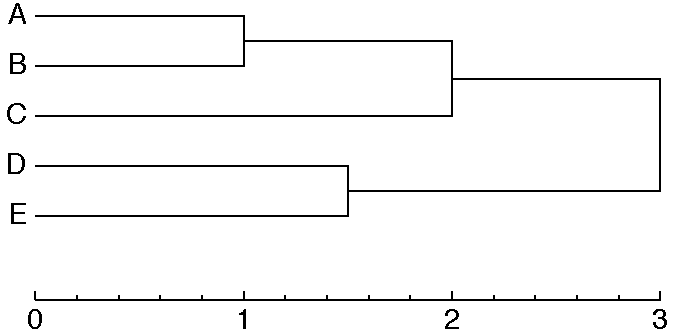
\includegraphics[width=0.75\linewidth]{fig-dendro.pdf}
\end{center}


\end{frame}
%===========================================================


%===========================================================
\begin{frame}
  \frametitle{Generic Algorithm for Hierarchical Clustering}


\begin{enumerate}
  \item Calculate a dissimilarity matrix for the $n$ items
  
  \item Join the two nearest items, $i$ and $j$

\begin{alertenv}
  \item Delete the $i$-th and $j$-th rows and columns of the dissimilarity matrix; and a new row/column that represents the dissimilarity of a new group ($i$,$j$) to all other items 
\end{alertenv}  

  \item Repeat from step 2 until there is a single group
\end{enumerate}

\begin{block}{Key Point}
 The different hierarchical clustering methods are determined by the function used to calculate the distance between groups in step 3.
\end{block}

\end{frame}
%===========================================================

%===========================================================
\begin{frame}
  \frametitle{Single Linkage Clustering}

\begin{block}{Group Distance Measure}
  Let $i$ and $j$ be groups, and $n_i$ and $n_j$ be the number of objects in the respective groups. 

  \smallskip

  $D_{ij}$ is the \emph{smallest} of the $n_i n_j$ dissimilarities between each element of $i$ and each element of $j$
\end{block}

Properties of Single Linkage Clustering
\begin{itemize}

\item Invariant under monotonic transformation of the $d_{ij}$

\item Unaffected by ties

\item Provably nice asymptotic properties

\item Disadvantage: susceptible to chaining

\end{itemize}

\end{frame}
%===========================================================


%===========================================================
\begin{frame}
  \frametitle{Hierarchical Clustering, Single Linkage Example}

\begin{center}
Step 1: Calculate Distance Matrix
\end{center}


\begin{columns}[t]

\begin{column}{0.5\linewidth}
Step 2: Find closest elements

\medskip

\begin{tabular}{c|ccccc}
  & A & B & C & D & E \\
\hline
A & 0 &   &   &   &    \\
B & 4 & 0 &   &   &    \\
C & \circled{1} & 4 & 0 &   &    \\
D & 4 & 2 & 4 & 0 &    \\
E & 5 & 5 & 3 & 4 &  0  \\
\end{tabular}
\end{column}

\begin{column}{0.5\linewidth}
Step 3: Update distance matrix

\medskip

\begin{tabular}{c|cccc}
& (A,C) & B & D & E \\
\hline
(A,C)& 0   &   &   &   \\
B    & 4   & 0 &   &   \\
D    & 4   & 2 & 0 &   \\
E    & 3   & 5 & 4 & 0 \\
\end{tabular}
\end{column}

\end{columns}

\end{frame}
%===========================================================

%===========================================================
\begin{frame}
  \frametitle{Worked Example, cont.}

\begin{center}
Repeat from Step 2
\end{center}

\begin{columns}[T]

\begin{column}{0.5\linewidth}
\begin{tabular}{c|cccc}
& (A,C) & B & D & E \\
\hline
(A,C)& 0   &   &   &   \\
B    & 4   & 0 &   &   \\
D    & 4   & \circled{2} & 0 &   \\
E    & 3   & 5 & 4 & 0 \\
\end{tabular}
\end{column}

\begin{column}{0.5\linewidth}
\begin{tabular}{c|ccc}
  & (A,C) & (B,D) & E \\
\hline
(A,C)& 0   &   &   \\
(B,D)& 4   & 0 &   \\
E    & 3   & 4 & 0 \\
\end{tabular}
\end{column}

\end{columns}


\begin{center}
Repeat from Step 2
\end{center}

\begin{columns}[T]

\begin{column}{0.5\linewidth}
\begin{tabular}{c|ccc}
  & (A,C) & (B,D) & E \\
\hline
(A,C)& 0   &   &   \\
(B,D)& 4   & 0 &   \\
E    & \circled{3}   & 4 & 0 \\
\end{tabular}
\end{column}

\begin{column}{0.5\linewidth}
\begin{tabular}{c|ccc}
  & ((A,C),E) & (B,D)  \\
\hline
((A,C),E) & 0   &   &   \\
(B,D)     & 4   & 0 &   \\
\end{tabular}
\end{column}

\end{columns}

\end{frame}
%===========================================================

%===========================================================
\begin{frame}
  \frametitle{Worked Example, cont.}

\begin{center}
Repeat from Step 2
\end{center}

\begin{columns}[T]

\begin{column}{0.5\linewidth}
\begin{tabular}{c|ccc}
  & ((A,C),E) & (B,D)  \\
\hline
((A,C),E) & 0   &   &   \\
(B,D)     & \circled{4}   & 0 &   \\
\end{tabular}
\end{column}

\begin{column}{0.5\linewidth}
\begin{tabular}{c}
Final Join \\
\hline
(((A,C),E),(B,D))
\end{tabular}
\end{column}

\end{columns}

\begin{figure}
\centering
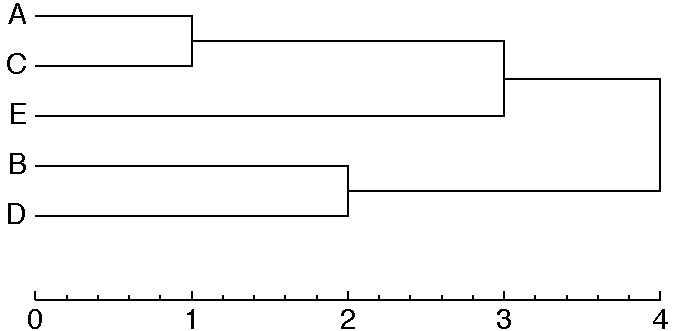
\includegraphics[width=0.5\linewidth]{fig-workedexample.pdf}
\caption{Final dendrogram for worked example}
\end{figure}

\end{frame}
%===========================================================



%===========================================================
\begin{frame}
  \frametitle{More Hierarchical Clustering Functions}


\begin{description}

\item[Complete Linkage] -- $D_{ij}$ is the maximum of the $n_i n_j$ dissimilarities between the two groups.

\item[Group Average Methods] -- $D_{ij}$ is the average of the $n_i n_j$  dissimilarities between the two group (UPGMA, WPGMA)

\item[Centroid Method] -- $D_{ij}$ is the squared Euclidean distance between the centroids of groups $i$ and $j$

\end{description}

\end{frame}
%===========================================================



%===========================================================
\begin{frame}[plain,c]
\begin{center}
\Huge K-means Clustering
\end{center}
\end{frame}
%===========================================================

%===========================================================
%% K-means clustering

\begin{frame}
\frametitle{K-mean Clustering}

\begin{block}{General idea}
Assign the $n$ data points (or $p$ variables) to one of $K$ clusters to as to optimize some criterion of interest.    
\end{block}

\begin{columns}
    
\begin{column}{5cm}
\begin{itemize}
\item The most common criterion to minimize is the sum-of-squares from the group centroids.

\[
V = \sum_{i=1}^k \sum_{j \in g_i}|x_j-\mu_i|^2
\]
\end{itemize}
\end{column}

\begin{column}{5.5cm}
\begin{center}
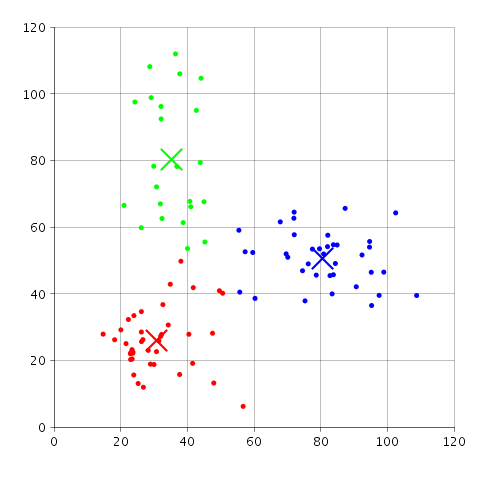
\includegraphics[width=0.9\textwidth]{k-means-simple.png}    
\end{center}
\end{column}

\end{columns}


\end{frame}
%===========================================================

%===========================================================
\begin{frame}
\frametitle{Simple algorithm for K-means clustering}

\begin{enumerate}
\item Decide on $k$, the number of groups

\item Randomly pick $k$ of the objects to act as the initial centers

\item Assign each object to the group whose center it is closest to

\item Recalculate the $k$ centers as the centroids of the objects assigned to them

\item Repeat from step 3 until centroids no longer move (convergence)

\end{enumerate}

\end{frame}
%===========================================================

%===========================================================
\begin{frame}
\frametitle{Illustration of K-means algorithm}
\begin{center}
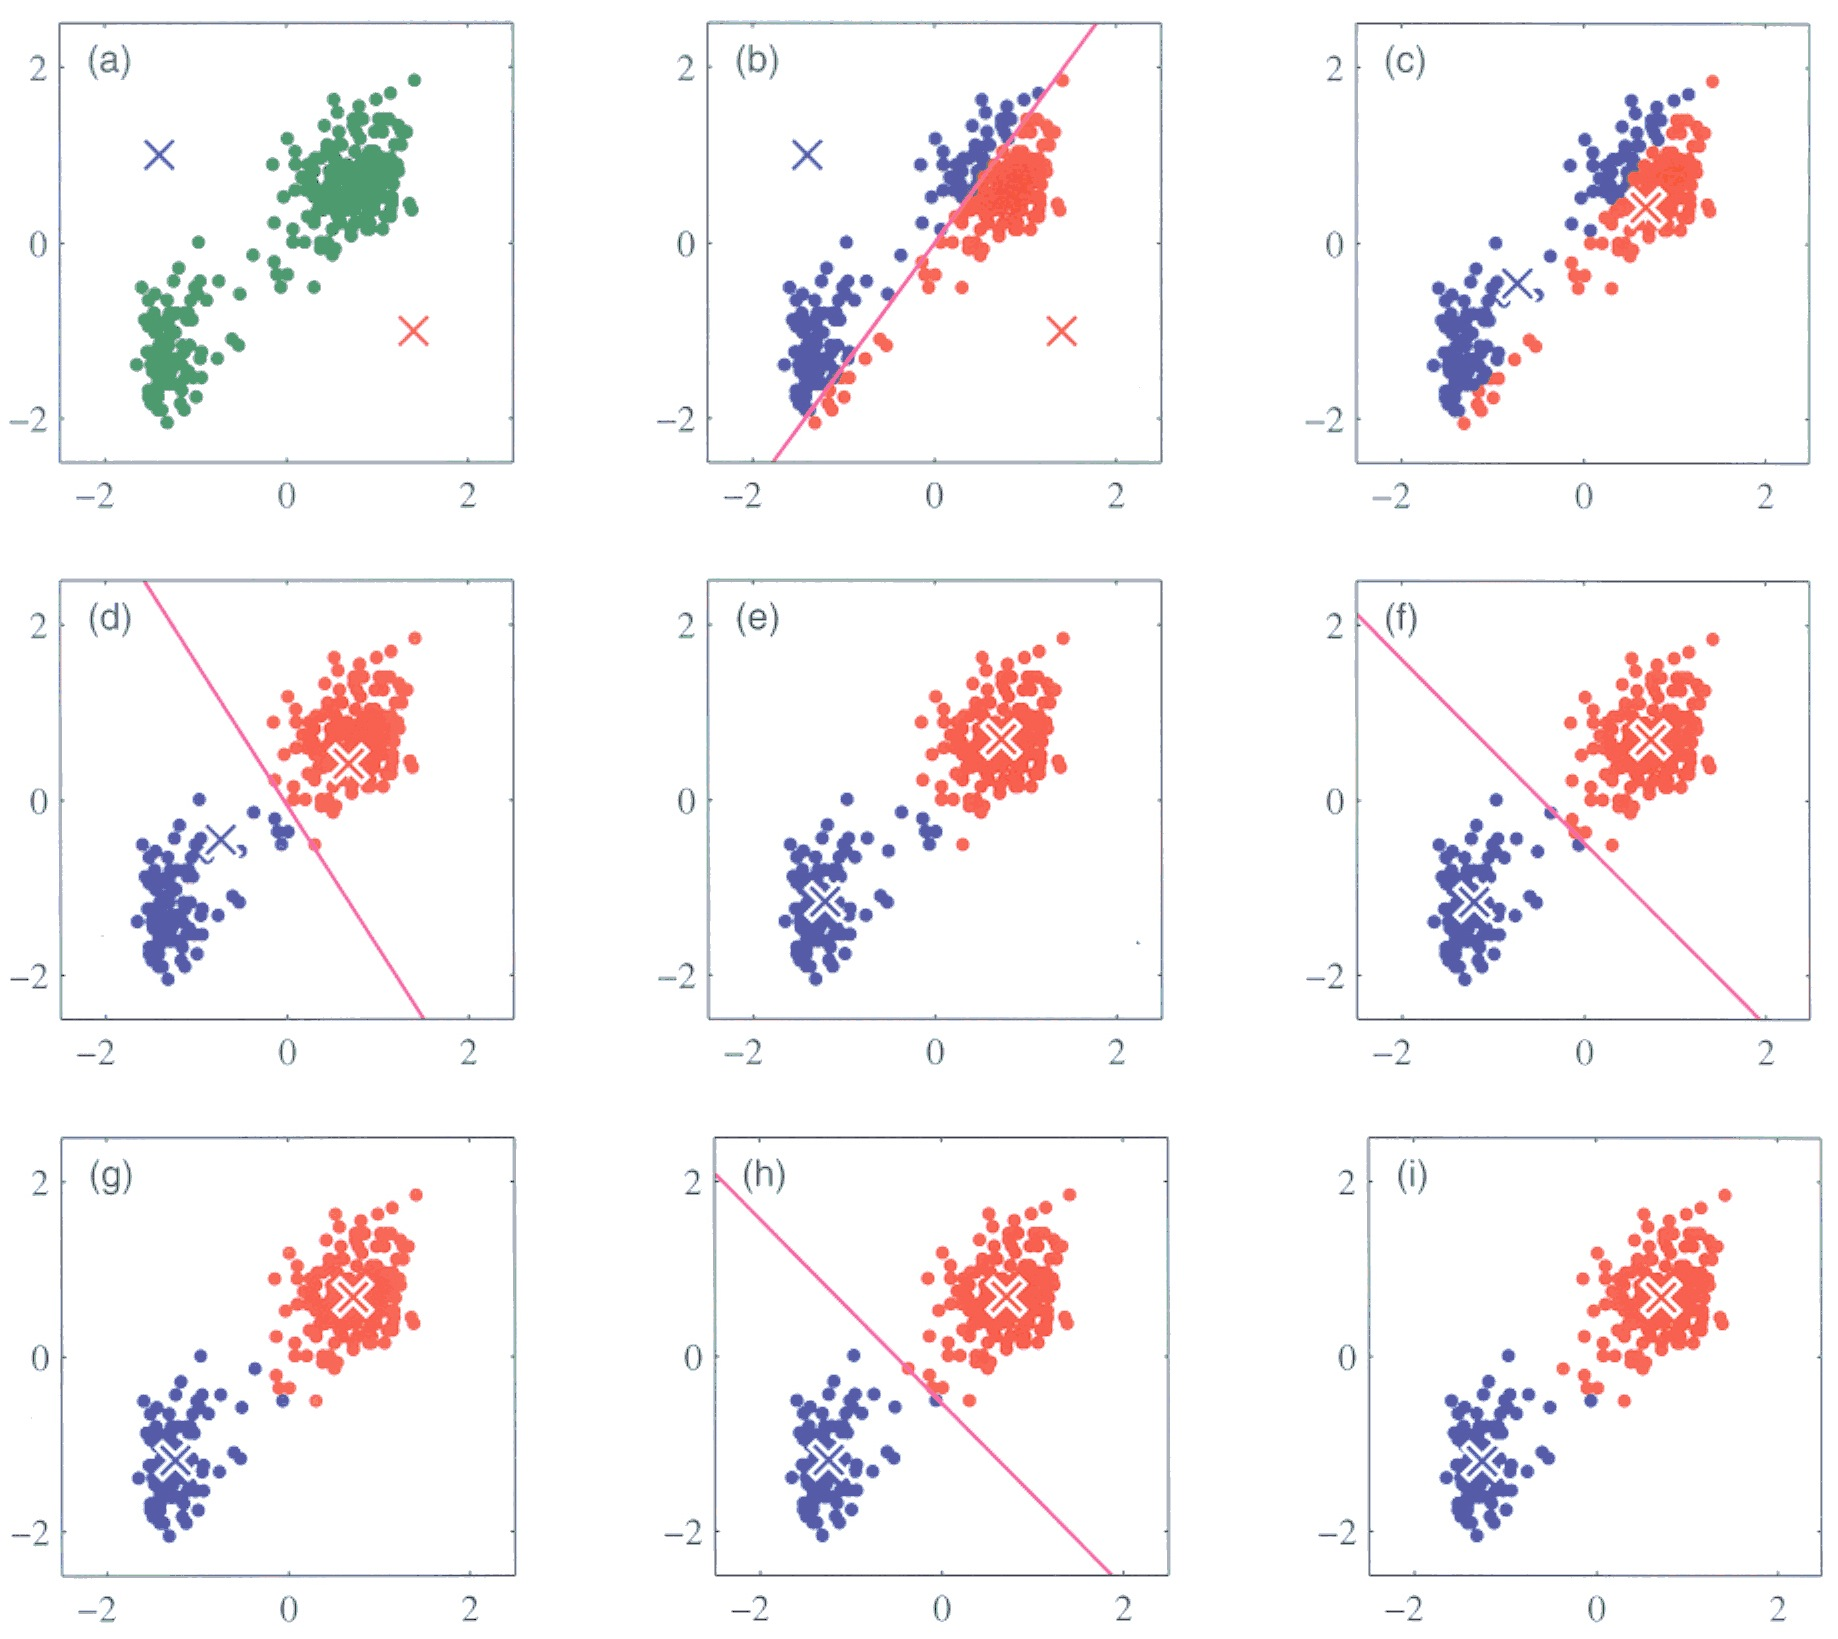
\includegraphics[height=3.2in]{k-means-fig.jpg}    
\end{center}
\end{frame}
%===========================================================

%===========================================================
\begin{frame}
\frametitle{Things to note re: K-means clustering}
\begin{itemize}
\item The algorithm described above does not necessarily find the global optimum

\bigskip

\item The algorithm is sensitive to choice of initial cluster center; k-means is often run multiple-time with different initial centers to insure inferred clusters are robust.    
\end{itemize}
\end{frame}
%===========================================================



\end{document}



%===========================================================
\begin{frame}
  \frametitle{XXX}

\end{frame}
%===========================================================



%%% Local Variables:
%%% mode: latex
%%% TeX-master: t
%%% TeX-command-extra-options: "-shell-escape" 
%%% End:
